\documentclass[]{elsarticle} %review=doublespace preprint=single 5p=2 column
%%% Begin My package additions %%%%%%%%%%%%%%%%%%%
\usepackage[hyphens]{url}

  \journal{Geographical Analysis} % Sets Journal name


\usepackage{lineno} % add
\providecommand{\tightlist}{%
  \setlength{\itemsep}{0pt}\setlength{\parskip}{0pt}}

\usepackage{graphicx}
\usepackage{booktabs} % book-quality tables
%%%%%%%%%%%%%%%% end my additions to header

\usepackage[T1]{fontenc}
\usepackage{lmodern}
\usepackage{amssymb,amsmath}
\usepackage{ifxetex,ifluatex}
\usepackage{fixltx2e} % provides \textsubscript
% use upquote if available, for straight quotes in verbatim environments
\IfFileExists{upquote.sty}{\usepackage{upquote}}{}
\ifnum 0\ifxetex 1\fi\ifluatex 1\fi=0 % if pdftex
  \usepackage[utf8]{inputenc}
\else % if luatex or xelatex
  \usepackage{fontspec}
  \ifxetex
    \usepackage{xltxtra,xunicode}
  \fi
  \defaultfontfeatures{Mapping=tex-text,Scale=MatchLowercase}
  \newcommand{\euro}{€}
\fi
% use microtype if available
\IfFileExists{microtype.sty}{\usepackage{microtype}}{}
\bibliographystyle{elsarticle-harv}
\usepackage{graphicx}
% We will generate all images so they have a width \maxwidth. This means
% that they will get their normal width if they fit onto the page, but
% are scaled down if they would overflow the margins.
\makeatletter
\def\maxwidth{\ifdim\Gin@nat@width>\linewidth\linewidth
\else\Gin@nat@width\fi}
\makeatother
\let\Oldincludegraphics\includegraphics
\renewcommand{\includegraphics}[1]{\Oldincludegraphics[width=\maxwidth]{#1}}
\ifxetex
  \usepackage[setpagesize=false, % page size defined by xetex
              unicode=false, % unicode breaks when used with xetex
              xetex]{hyperref}
\else
  \usepackage[unicode=true]{hyperref}
\fi
\hypersetup{breaklinks=true,
            bookmarks=true,
            pdfauthor={},
            pdftitle={A spatio-temporal analysis of the environmental correlates of COVID-19 incidence in Spain},
            colorlinks=false,
            urlcolor=blue,
            linkcolor=magenta,
            pdfborder={0 0 0}}
\urlstyle{same}  % don't use monospace font for urls

\setcounter{secnumdepth}{5}
% Pandoc toggle for numbering sections (defaults to be off)


% Pandoc header
\usepackage{booktabs}
\usepackage{longtable}
\usepackage{array}
\usepackage{multirow}
\usepackage{wrapfig}
\usepackage{float}
\usepackage{colortbl}
\usepackage{pdflscape}
\usepackage{tabu}
\usepackage{threeparttable}
\usepackage{threeparttablex}
\usepackage[normalem]{ulem}
\usepackage{makecell}
\usepackage{xcolor}



\begin{document}
\begin{frontmatter}

  \title{A spatio-temporal analysis of the environmental correlates of COVID-19
incidence in Spain}
    \author[Some School]{Author A\corref{1}}
   \ead{author.a@example.com} 
    \author[Some Institute]{Author B}
   \ead{author.b@example.com} 
      \address[Some School]{School of the Things}
    \address[Some Institute]{Institute of Everything}
    \address[Departamento de Economia]{}
      \cortext[1]{Corresponding Author}
  
  \begin{abstract}
  The novel SARS-CoV2 has disrupted health systems and the economy and
  public health interventions to slow its spread have been costly. How and
  when to ease restrictions to movement hinges in part on whether
  SARS-CoV2 will display seasonality due to variations in temperature,
  humidity, and hours of sunshine. Here, we address this question by means
  of a spatio-temporal analysis in Spain of the incidence of COVID-19, the
  disease caused by the virus. Use of spatial Seemingly Unrelated
  Regressions (SUR) allows us to model the incidence of reported cases of
  the disease per 100,000 population as an interregional contagion
  process, in addition to a function of temperature, humidity, and
  sunshine. In the analysis we also control for GDP per capita, percentage
  of older adults in the population, population density, and presence of
  mass transit systems. The results support the hypothesis that incidence
  of the disease is lower at higher temperatures and higher levels of
  humidity. Sunshine, in contrast, displays a positive association with
  incidence of the disease. Our control variables also yield interesting
  insights. Higher incidence is associated with higher GDP per capita and
  presence of mass transit systems in the province; in contrast,
  population density and percentage of older adults display negative
  associations with incidence of COVID-19.
  \end{abstract}
  
 \end{frontmatter}

\hypertarget{introduction}{%
\section{Introduction}\label{introduction}}

From a small outbreak linked to a live animal market at the end of 2019
to a global pandemic in a matter of weeks, the SARS-CoV2 virus and
COVID-19, the disease it causes, have threatened to overrun health
systems around the world. In efforts to contain the spread of the
disease, numerous governments in many regions and nations have either
recommended or mandated social distancing measures, and as of this
writing, millions of people in five continents shelter in place. There
are encouraging signs that these measures have mitigated the spread of
the virus (e.g., Lancastle, 2020; Lewnard and Lo, 2020; Wilder-Smith and
Freedman, 2020). Even so, this has come at a high cost, and the
consequences for all spheres of economic, social, and cultural life have
been dire (e.g., Fernandes, 2020; Luo and Tsang, 2020). As a result,
there is a sense of urgency to anticipate the progression of the
pandemic, in order to plan for progressive lifting of restrictions to
movement and social contact (e.g., Kissler et al., 2020). Needless to
say, this has become a delicate, and politically charged, balancing act
between public health and the economy (Gong et al., 2020).

A salient question in the debate about how and when to ease social
distancing measures is whether the virus will display seasonal
variations. Existing research on similar pathogens suggests that the
virus could be more stable and potentially easier to transmit in
conditions of low temperature and low humidity. While this is
encouraging, it is important to keep in mind that ``not all seasonal
respiratory viruses experience the same spatiotemporal patterns'' (Ángel
Solá et al., 2020, sec. 4). This urges caution when extrapolating from
known viruses. The evidence in this respect is as yet inconclusive, and
although easing restrictions as the weather warms may appear tempting,
doing so prematurely could well undo weeks or possibly months of costly
measures.

It is not surprising, given the stakes involved, that this issue has
already triggered a lively debate. The current state of knowledge was
well-summarized by the National Academy of Sciences, Engineering, and
Medicine in the U.S. in a recent report (see National Academies of
Sciences, Engineering and Medicine, 2020). Engaged by the Office of the
Executive for guidance on this matter, this organization concluded that:
``{[}some{]} limited data support a potential waning of cases in warmer
and more humid seasons, yet none are without major
limitations\ldots Additional studies as the SARS-CoV2 pandemic unfolds
could shed more light on the effects of climate on transmission''
(p.~6). To further complicate matters, much of the relevant work has yet
to be peer-reviewed (see for instance the challenge of Harbert et al.,
2020; to Araujo and Naimi, 2020).

With the above considerations in mind, our objective with this paper is
to investigate the influence of environmental factors, concretely
temperature, humidity, and sunshine, on the progression of the pandemic.
We adopt a population health approach, and report results from a
spatio-temporal model of the incidence of COVID-19 in the coterminous
provinces in Spain, one of the countries hardest hit by the pandemic. We
combine data on reported cases of the disease with metereological
information, to create a spatio-temporal dataset covering a period of 30
days. We then join this dataset with provincial-level economic and
demographic information to act as controls to our key environmental
variables. These data are analyzed using a spatial Seemingly Unrelated
Regressions (SUR) approach, which allows us to model incidence of
COVID-19 as a contagion process.

The results provide evidence of the effect of temperature, humidity, and
sunshine on the incidence of COVID-19. The clearest result with respect
to these variables is a lower incidence of COVID-19 at higher
temperatures and levels of humidity, while the opposite happens with
respect to hours of sunshine. Our control variables also provide some
intriguing insights. Higher incidence is associated with higher GDP per
capita and presence of mass transit systems in the province; in
contrast, population density and percentage of older adults display
negative associations with incidence of COVID-19. The results of this
analysis provide support to the hypothesis of seasonality of the novel
SARS-CoV2, and should be of interest to public health officials and
policy makers grappling with the question of the trajectory of the
pandemic.

Please note that this paper is prepared as a reproducible research
document. The source \texttt{R} markdown document, as well as all data
and code needed to reproduce/review/extend the analysis can be obtained
from a public
repository\footnote{\url{https://drive.google.com/drive/u/1/folders/1d_40N_QXo2Fl14r3T3CHs84IED-B1rV_}}.

\hypertarget{background}{%
\section{Background}\label{background}}

The global emergence of infectious diseases is mostly driven by
environmental, ecological, and socio-economic factors (Jones et al.,
2008). In the case of SARS-CoV2, the ecological factors include the
interaction between humans and wildlife. Once transmission of a disease
begins to happen between humans, socio-economic and environmental
factors become increasingly important. As noted in the introduction, the
focus of the paper is on environmental variables, concretely three
related to meteorological conditions: temperature, humidity, and
sunshine.

Much of what is known about the potential seasonality of SARS-CoV2 is a
result of research on other pathogens. Earlier, diverse studies have
shown the effect of temperature and humidity on the incidence of
influenza (e.g., Mäkainen et al., 2009; Jaakkola et al., 2014; Kudo et
al., 2019). Jaakkola et al.~(2014), for example, found that a decrease
of temperature and absolute humidity precedes the onset of symptoms of
influenza A and B viruses by 3 days in places where the temperature is
low. After the 2002-2004 outbreak of SARS, researchers also began to
investigate the relationship between these factors and SARS-CoV
(Casanova et al., 2010; Chan et al., 2011). Casanova et al.~(2010), for
instance, used surrogates to find that virus inactivation was likely
more rapid at higher temperatures; in terms of humidity, these
researchers reported that survival of the virus was lower at moderate
relative humidity levels. Chan et al.~(2011) also found that viability
of the virus that causes SARS is also lost at higher temperatures
(\textgreater38°C) and relative humidity superior to 95\%.

Whether results from laboratory experiments will hold when the virus
circulates in the community remains uncertain. At a global scale, de
Ángel Solá et al.~(2020) see less risk from SARS-CoV2 in the Caribean
Basin; on the other hand, Coelho et al.~(Coelho et al., 2020) warn that
at least during the exponential phase, expansion of the virus is not
driven by climate. Similarly, whereas Araujo and Naimi (2020) argue that
spread of SARS-CoV2 will likely be constrained by climate, Harbert et
al.~(2020) remain unconvinced that spatial modelling can currently
discriminate the distribution of the disease on the basis of climate, at
least in the United States. Yao et al.~(2020), examined data from China
and came to the conclusion that neither temperature nor ultraviolet
indices had an association with transmission of COVID-19. This is
despite previous research that has linked less exposure to UVB radiation
to higher prevalence and severity of acute respiratory tract infections
(Zittermann et al.~2016; Dąbrowska-Leonik et al.~2018; Dinlen et
al.~2016; Mathyssen et al.~2017; Esposito and Lelii 2015; Jat 2017;
Moriyama, Hugentobler, and Iwasaki 2020).

In addition to the environmental variables above, from a population
health perspective it is also important to account for potential
socio-economic and demographic confounders.

To account for population-level factors, the first variable that we
consider is GDP per capita. Much has been written about globalization
and the spread of infectious
disease\footnote{As the Globe and Mail, Canada's paper of record, put it in relation to the SARS outbreak in 2003: "Globalization means that if someone in China sneezes, someone in Toronto may one day catch a cold" (Editorial, March 28, 2003, p. A18)}.
The growth in global connections has presented a challenge to spatial
approaches in the initial stages of disease management, when the cause
of a disease may still be unclear but the plane has already departed
(Zhou and Coleman, 2016). In reference to the earlier outbreak of SARS,
van Wagner (2008) chronicles how Toronto's status as a global city
turned out to be a vulnerability in this respect. In our case, we think
of GDP per capita as a marker of a region's relative position in a
network of global cities, and its potential to be further ahead in the
trajectory of the pandemic. Furthermore, wealthier regions also tend to
concentrate more activities that produce non-traded goods, including
building and construction (Hallet, 2002). Therefore, it is possible that
wealthier regions remain relatively more active even during a lockdown.
On the other hand, we cannot discount the possibility that less wealthy
regions have a higher proportion of workers in manual occupations who
cannot telework, and therefore have more difficulties complying with
shelter-in-place orders.

Secondly, we consider percentage of older adults (over 65) in a region.
Early evidence regarding COVID-19 suggests that the case rate mortality
is higher at older ages (e.g.~The Novel Coronavirus Pneumonia Emergency
Response Epidemiology Team, 2020). However, it is not clear that a
relatively large population of older adults necessarily translates into
higher transmission rates of the infection. The tool of choice in
containing the spread of the disease has been social distancing. In this
respect, the evidence from the field of transportation is that older
adults tend to travel less frequently, for shorter distances, and have
higher rates of immobility than most everyone, except the youngest
members of the public (e.g., Roorda et al., 2010; Morency et al., 2011;
Sikder and Pinjari, 2012). In other words, many older adults are,
whether by preference or otherwise, already in a form of social
isolation. Social distancing during the pandemic may actually reinforce
that condition for them, as suggested by the analysis of age-structured
social contact in India, China, and Italy of Sing and Adhikari (2020).
Since the age-structured matrix of social contact in Spain is similar to
Italy (see Prem et al., 2017), our expectation is that populations with
higher percentages of older adults will tend to have lower levels of
social contact and hence of incidence.

Population density is also relevant since it directly affects the
contact patterns and contact rates between individuals in a population
(Hu et al., 2013). The evidence available suggests a positive
relationship between the transmission of COVID-19 and population density
(e.g.~cumulative incidence in urban areas like NYC). For this reason, we
anticipate a positive relationship between population density and the
incidence of the disease.

The last variable that we consider as a control is the presence of mass
transit systems in a province. Every province in Spain offers some form
of public transportation, but only five provinces have higher order
systems of mass mobility (e.g.~metro or subway), namely Barcelona,
Madrid, Sevilla, Valencia, and Bizkaia. Public transportation has been
hypothesized to relate to the spread of contagious disease by some
researchers using agent-based approaches and simulation (e.g., Perez and
Dragicevic, 2009; Wang et al., 2010), and while we find scant evidence
of a link in the literature, the idea is intuitively appealing. After
all, unlike the isolation that a car offers to travellers, most mass
transit system are cauldrons of social contact.

\hypertarget{context-and-data}{%
\section{Context and Data}\label{context-and-data}}

\hypertarget{covid-19-in-spain}{%
\subsection{Covid-19 in Spain}\label{covid-19-in-spain}}

The first reported case of COVID-19 in Spain was on January 31st, 2020,
when a German tourist in the Canary Islands tested positive for the
virus. After this case, it was still a few weeks before the first
domestic case was reported, on February 27th in Sevilla province
(Andalusia). In a short period of time, as testing started to ramp up,
it became clear that an outbreak was flaring. By March 11th the World
Health Organization (WHO) declared COVID-19 officially a pandemic. This
declaration marked a turning point for the public in Spain too. As of
March 13th, the number of cases of COVID-19 reported in Spain was 4,473,
with a majority of cases (1,990) concentrated in Madrid: these numbers
were at the time the worst outbreak in Europe after Italy. In response
to the situation, on March 13th the Spanish National Government declared
a state of emergency, to go into effect on Saturday March 14th. As part
of the state of emergency restrictions to most activities were imposed,
with the exception of essential services (e.g.~food, health) and some
economic subsectors of industry and construction. A few days later, on
March 17th, Spain closed its lands borders to allow entry only to
returnee nationals and permanent residents. The lockdown was further
hardened between March 30th and April 12th (including the Easter weekend
of April 10th-12th) and during this period only essential activities
were allowed. During this period, there was a dramatic reduction in
overall mobility, both within provinces as between
\footnote{https://www.mitma.gob.es/ministerio/covid-19/evolucion-movilidad-big-data/movilidad-provincial}.

\hypertarget{data}{%
\subsection{Data}\label{data}}

Our dataset includes information about the daily number of cases of
COVID-19 reported in Spain at the provincial level (NUTS3 in Eurostat
terminology) for the period between March 13th and April 11th,
inclusive. For our purposes, we consider positive cases reported, but
exclude symptomatic cases diagnosed by a doctor without a Polymerase
Chain Reaction (PCR) test. The Spanish National Government publishes
periodic updates at the regional level (NUTS2) and the information is
also released at the provincial level as part of a collaborative project
by geovoluntarios.com\footnote{https://www.geovoluntarios.org/},
ProvidencialData19\footnote{https://www.datoscovid.es/pages/providencialdata19},
and ESRI España. This information is compiled from several sources,
mainly the official web pages of the Spanish regional goverments, as
documented in Centro de Datos
Covid-19\footnote{https://www.datoscovid.es/pages/sobre-la-iniciativa}.
We consider two sets of explanatory variables. The first one, and the
focus of this research, are the three environmental variables, collected
from official sources (i.g., \emph{AEMET}, the state meteorology agency,
and \emph{MAPA}, the ministry of agriculture, fisheries, and food). The
second set provides some relevant controls as discussed above, and are
also collected from official sources, i.e., INE, the national statistics
institute. Table \ref{tab:descriptive-statistics} shows the descriptive
statistics and the provenance of the data used in this research.

The spatial and temporal coverage of the data is as follows. Our dataset
begins on March 13, which is the first date when every province had
reported at least one case of COVID-19, and continues until April 11,
for a period of 30 days. The unit of analysis is the province. Provinces
are the equivalent of states, and are embedded in Autonomous
Communities. As an example, Cataluña is an Autonomous Community and
consists of four provinces, namely Barcelona, Gerona, Lerida, and
Tarragona. The size of the provinces is relatively large, as seen in
Table \ref{tab:descriptive-statistics}. The smallest province is
\(1,978.12km^2\) (this is smaller than Rhode Island in the U.S.) and the
largest province is \(21,767.93km^2\) (slightly smaller than New Jersey
in the U.S.). While this is a relatively large degree of spatial
aggregation, reporting on COVID-19 is not yet consistent at smaller
geographies, or cases are not reported at that level at all.

\begin{table}

\caption{\label{tab:descriptive-statistics}\label{tab:descriptive-statistics} Descriptive statistics}
\centering
\resizebox{\linewidth}{!}{
\begin{tabular}[t]{l>{\raggedright\arraybackslash}p{15em}rrrr>{\raggedright\arraybackslash}p{5em}}
\toprule
Variable & Note & Min & Mean & Max & SD & Source\\
\midrule
\rowcolor{gray!6}  COVID-19 Incidence & Incidence in reported cases of SARS-19 per 100,000 people & 0.38 & 153.61 & 1149.36 & 186.23 & ProvidencialData19\\
Area & Area of province in sq.km & 1978.12 & 10118.79 & 21767.93 & 4.77 & INE\\
\rowcolor{gray!6}  GDPpc & GDP per capita in €1,000s & 16.67 & 22.51 & 36.00 & 4805.98 & INE\\
Older & Percentage of people aged 65 and older in the province & 15.16 & 21.03 & 31.36 & 3.95 & INE\\
\rowcolor{gray!6}  Population Density & Population density in the province in people per sq.km & 8.60 & 140.04 & 829.76 & 181.25 & INE\\
\addlinespace
Mean Temperature & Mean temperature in province by date, in °C & 1.00 & 12.18 & 23.20 & 3.67 & AEMET\\
\rowcolor{gray!6}  Humidity & Relative humidity in province by date & 2.00 & 77.82 & 100.00 & 10.37 & MAPA\\
Sunshine & Daily hours of sunshine in province by date & 0.00 & 5.74 & 12.40 & 3.96 & AEMET\\
\bottomrule
\multicolumn{7}{l}{\textit{Note: }}\\
\multicolumn{7}{l}{ProvidencialData19: https://www.datoscovid.es/pages/providencialdata19}\\
\multicolumn{7}{l}{INE (Instituto Nacional de Estadistica): https://www.ine.es/}\\
\multicolumn{7}{l}{AEMET (Agencia Estatal de Meteorologia): http://eportal.mapa.gob.es}\\
\multicolumn{7}{l}{MAPA (Ministerio de Agricultura, Pesca y Alimentacion): http://eportal.mapa.gob.es}\\
\end{tabular}}
\end{table}

An important aspect of working with environmental data such as
temperature, humidity, and hours of sunshine, is the incubation period
of the disease. Lauer et al.~(2020) report for the case of COVID-19 a
median incubation period of 5.7 days (with a confidence interval between
4.9 to 7.8 days). The vast majority of cases (95\%) develop symptoms
between 2.6 days (CI, 2.1 to 3.7 days) and 12.5 days (CI, 8.2 to 17.7
days). For this reason, we judge it best to use lagged values of the
environmental variables. We test different time lags as follows. We
consider a lagged 8-day average, from date-minus-12 to date-minus-5 days
(hereafter \emph{lag8}). Secondly, we consider a lagged 11-day average,
from date-minus-12 to date-minus-2 days (hereafter \emph{lag11}).
Finally, to account for the likely duration of incubation, we consider a
lagged 11-day \emph{weighted} average, from date-minus-12 to
date-minus-2 days (hereafter \emph{lag11w}). The weights for this
variable are calculated using the parameters of the log-normal
distribution reported by Lauer et al.~(2020), i.e., a log-mean of 1.621
and a log-standard deviation of 0.418. With these weights, the
environmental variables at date-minus-2 and date-minus-12 days are
weighted as 0.041 and 0.009 respectively, whereas the environmental
variables at date-minus-5 days are weighted as 0.194. These weights have
the effect of changing the contribution of daily values to the lagged
moving average. For instance, the temperature at date-minus-4-days is
weighted more heavily than the temperature at date-minus-10-days, as a
closer approximation of the conditions at the most likely time of
contagion before the disease became manifest.

\hypertarget{methods}{%
\section{Methods: the Spatial SUR Model}\label{methods}}

The Seemingly Unrelated Regression equations model (SUR hereafter) is a
multivariate econometric model used in different fields when the
structure of the data consists of cross-sections for different time
periods. The basis of this approach is well-known since the initial
works of Zellner (1962), and has become a popular methodology included
in several econometrics textbook (e.g., Greene, 2003). To our knowledge,
Anselin (1988) was the first author to discuss SUR from a spatial
perspective, in the context of spatio-temporal analysis. In his landmark
text, Anselin discussed a model made of ``an equation for each time
period, which is estimated for a cross section of spatial units''
(p.~141). From this milestone, a large body of research has developed to
extend the classical SUR into a spatial framework (e.g., Rey and
Montouri, 1999; Lauridsen et al., 2010; Le Gallo and Dall'Erba, 2006;
López et al., 2017).

The classical SUR model without spatial effects (from here, SUR-SIM) is
a stack of equations as follows:

\begin{equation}
\label{eq:sur-sim}
\begin{bmatrix}
y_1 \\ y_2 \\ \vdots \\ y_T
\end{bmatrix}
=
  \begin{bmatrix}
X_1 & 0 & \cdots & 0 \\ 0 & X_2 & \cdots & 0 \\ \vdots & \vdots & \ddots & \vdots \\ 0 & 0 & \cdots & X_T
\end{bmatrix}
\
\begin{bmatrix}
\beta_1 \\ \beta_1 \\ \vdots \\ \beta_T
\end{bmatrix}
+
\begin{bmatrix}
\epsilon_1 \\ \epsilon_2 \\ \vdots \\ \epsilon_T
\end{bmatrix}
\end{equation}

\noindent where \(y_{t}=(y_{1t},...,y_{Nt})\) is a \(N \times 1\)
vector, and in our case \(y_{st}\) is the incidence ratio in the
province \(s\) (\(s=1,...,N\)) the day \(t\) \((t=1,...,T)\); \(X_t\) is
a \(N \times k_t\) matrix of the \(k_t\) independent variables, with
associated vector of coefficients \(\beta_t\),;
\(\beta_t=(\beta_{1t},...,\beta_{Nt})\) is a vector of coefficients and
\(\epsilon_t=(\epsilon_{1t},...,\epsilon_{Nt})\) is the vector of
residuals.

A key feature of the SUR model is the temporal dependence structure
among the vectors of residuals, namely:

\begin{equation}
\label{eq:sur-err}
E[\epsilon_t \epsilon'_{t'}]=\sigma_{tt'}
\end{equation}

Note that this specification is very flexible, in that it allows changes
in the coefficients \(\beta_{it}\) in order to modulate the effect of
the independent variables on \(y_t\). This flexibility can be reduced
and it is posible to impose restrictions considering some \(\beta\)
coefficients as being constant over time. In this case, we can
reformulate the coefficients expression
\(\beta_t = (\beta_{1}, \cdots, \beta_{r-1}, \beta_{r}, \beta_{r+1}, \cdots, \beta_{Nt})\)
to restrict the first \(r\) coefficients to be constant across
equations. This is equivalent to specifying some effects to be invariant
over time.

Equation (\ref{eq:sur-sim}) can be rewriten in compact form:

\begin{equation}
\bf{Y} = \bf{X} \beta + \epsilon
\label{eq:sur-sim-block}
\end{equation}

\noindent where \(\bf{Y}\) is now a vector of dimension \(NT \times 1\),
\(\bf{X}\) is a block-diagonal matrix \(NT \times K\) (with
\(K = \sum_t{k_t}\)) and \(\epsilon\) is an \(NT \times 1\) vector.
Using the Kronecker product notation (\(\otimes\)), the error matrix
structure is expressed concisely as:

\begin{equation}
E[\epsilon \epsilon']=\bf{\Sigma} \otimes \bf{I_N} ; \ \bf{\Sigma}=(\sigma_{tt'})
\end{equation}

As is the case with cross-sectional data, it is possible to test the
residuals of Model (\ref{eq:sur-sim-block}) for spatial autocorrelation,
and several tests have been developed to test the null hypothesis of
spatial independence (see López et al., 2014). When the null hypothesis
is rejected, several alternative specifications have been proposed to
include spatial effects (Anselin, 1988, see also 2016). In this paper we
consider a spatial SUR model that incorporates a spatial lag of the
dependent variable as an explanatory factor. Spatial analytical
approaches were used to understand contagion-difussion processes in the
case of infectious disease in general (e.g., Cliff et al., 1998) and the
2003-2004 SARS outbreak in particular (e.g., Meng et al., 2005; Cao et
al., 2010). While we are mindful of the same caveat that the novel
SARS-CoV2 may not follow the patterns of previous diseases, there is
still evidence from the United States that COVID-19 displays spatial
patterns that are consistent with a diffusion process (Desjardins et
al., 2020). For this reason, the spatial lag model is appropriate to
model incidence of COVID-19 geographically, since it accounts for
potential spatial patterns that result from a process of contagion, as
explained next.

The stack expresion for the SUR model with a spatially lagged dependent
variable (SUR-SLM) is as follows:

\begin{equation}
\label{eq:sur-slm}
\begin{aligned}
\bf{AY} = \bf{X} \beta + \epsilon \\
\epsilon =N(0,\bf{\Sigma})
\end{aligned}
\end{equation}

\noindent where \(\bf{A} =I_{TN}-\bf{\Gamma} \otimes W\) is the
spatially lagged dependent variable, and
\(\bf{\Gamma} = diag(\rho_1, \cdots, \rho_T)\).

This specification assumes that outcome (\(y_{st}\)) at location \(s\)
and time \(t\) is partially determined by the weighted average
(\(Wy_{st}\)) of the outcome in neighboring provinces, with neighborhood
defined by matrix \(W\) of spatial weights. In other words, the
spatially lagged dependent variable represents a process of contagion,
where the disease in neighboring provinces can spillover in a spatial
way. The coefficients of the spatially lagged variable are estimated for
each time period \(\rho_t\) and identify the intensity and the sign of
the contagion effect. It is possible test the null hypothesis of
identical levels of spatial dependence (\(\rho_i=\rho_j, \forall i,j\)).
The correspond Wald test is available in the \texttt{R} package
\texttt{spsur}.

The SUR-SLM model can be estimated using maximum likelihood (López et
al. (2014)) or instrumental variables (Mínguez et al. (2019)).

A note regarding the interpretation of the model is in order. It is
well-known that coefficients in linear regression models are partial
derivatives of the dependent variable with respect to the independent
variables, and therefore directly give the marginal effects or rates of
change. Spatially lagged models, however, are no longer linear. The
intuition behind the non-linearity is that the spatial lag expands the
information set to include information from neighbouring regions: in
other words, the value of an explanatory variable in a spatial unit can
have influence in other spatial units via the spatial lag. This makes
interpretation of the coefficients less straightforward but also richer
(Golgher and Voss, 2016). The results of LeSage (2009) for
cross-sectional spatial lag models can be extended to the spatial SUR
framework. Note that, according to Elhorst (2014), the partial
derivatives have the following interpretation: if an explanatory
variable (\(X_k\)) in a particular province changes, not only the
incidence rate in that province changes, also incidence rates in other
provinces change via the contagion effect. Therefore, a change in
\(X_k\) in a particular province has a \emph{direct effect} on that
province, but also an \emph{indirect effect} on neighbouring provinces.
In this way, the \(i\)th diagonal element of the matrix of partial
derivatives represents the direct effect on the \(i\)th province,
whereas the non-diagonal elements of \(i\)th row of the matrix of
partial derivatives represent the indirect effects on other provinces.
In order to obtain a global indicator, the direct effect is calculated
as the mean of the diagonal elements and captures the average change in
incidence ratio caused by the change in \(X_k\). Likewise, a global
indicator of the indirect effects is calculated as the mean of the
non-diagonal elements. The total effect is the sum of direct and
indirect effects. Finally, note that if \(\rho_k = 0\), the indirect
effects are 0 and the direct effects are equal to \(\beta_kt\).

\hypertarget{results}{%
\section{Results}\label{results}}

\hypertarget{eda}{%
\subsection{Exploratory Data Analysis}\label{eda}}

Figure \ref{fig:weekly-average-incidence-map} shows the geographical
variation in the incidence of COVID-19 in Spain, as well as the temporal
progression of the disease in weekly averages. Our analysis begins on
March 13. Albeit still low, the highest incidence at this early date was
in the provice of Álava, in the North of Spain. Álava is not the most
populous province, with a population of only 331,549, but it has the
highest GDP per capita of all provinces. Vitoria, its main city, is the
capital of the Basque Country and has been the focus of efforts, along
with San Sebastian and Bilbao, to develop a ``Global Basque City''
(Meijers et al., 2008). The other early focus of the pandemic in Spain
was Madrid, which is the most populous province in the country and has
the second highest GDP per capita after Álava. The early outbreaks in
these two provinces can be traced throughout the progression of the
pandemic over time, although by the end of the period under study, other
provinces had matched and even surpased their incidence rates, including
Segovia and Soria to the north of Madrid, and Ciudad Real and Albacete
to the south.

\begin{figure}
\centering
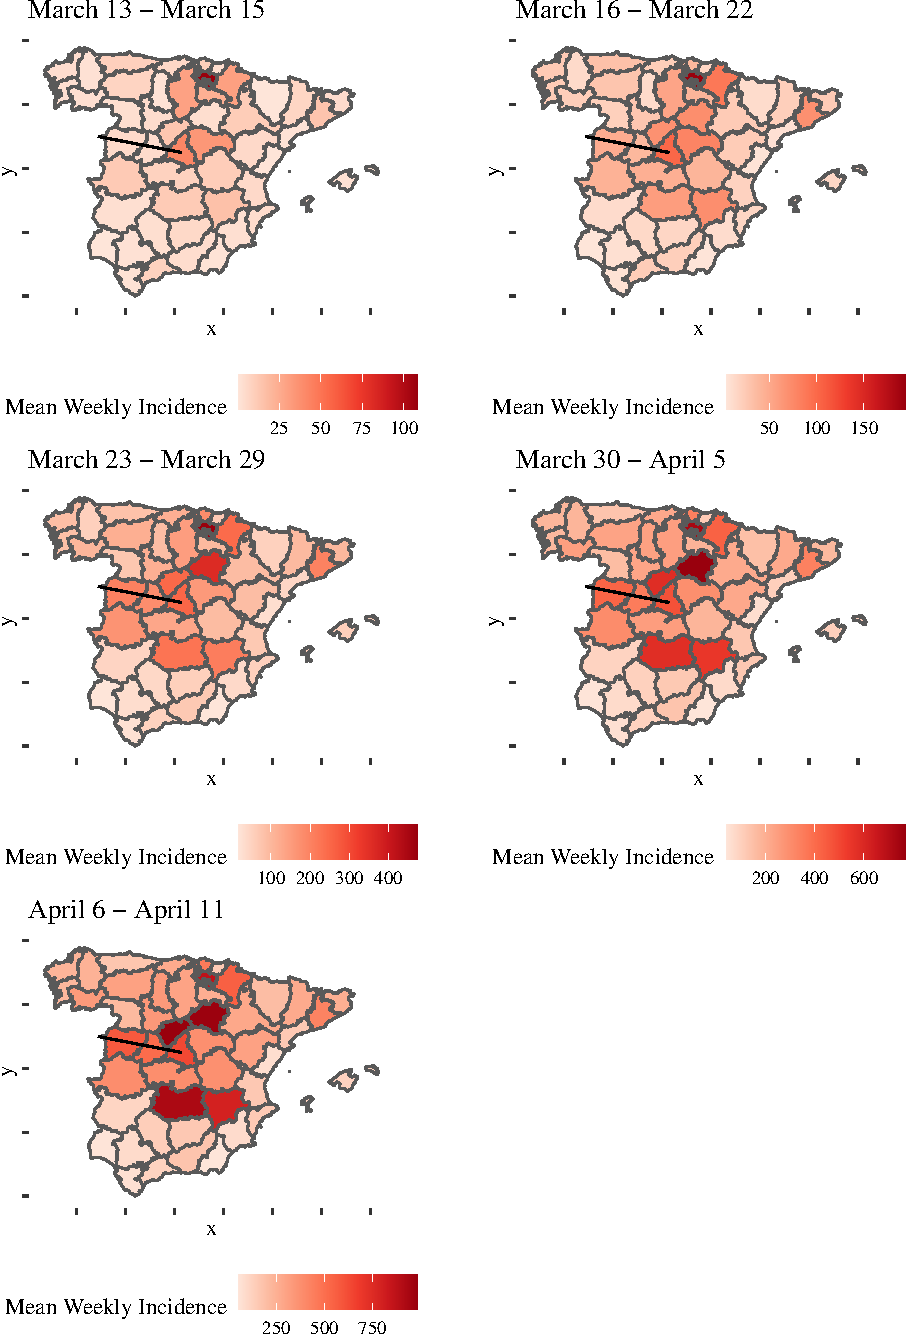
\includegraphics{Environmental-Correlates-of-COVID19-Spain_files/figure-latex/weekly-average-incidence-map-1.pdf}
\caption{\label{fig:weekly-average-incidence-map}Mean weekly incidence
of COVID-19 by province, in reported cases by 100,000 people}
\end{figure}

Figure \ref{fig:descriptives-temperature} shows the distribution of the
environmental variables in Spain. For ease of visualization we aggregate
the provinces by Autonomous Community. Each box-and-whisker in the
figure represents the distribution of the variable for a community over
the 30-day period. In the plot, the communities have been sorted by
latitude, so that Principado de Asturias is the northernmost community,
and Andalucia the southernmost. As seen in the figure, there is a
relatively wide range of values both within and between provinces over
the 30-day period examined. The top panel of the figure shows the
distribution of mean temperatures. The lowest mean temperature for a
community on any given day was approximately 3°C, and the highest about
20°C, for a range of approximately 17 degrees. Likewise, there is a
great deal of variability in humidity, as seen in the middle panel of
the figure, where the lowest mean humidity for any community is
approximately 48\% and the highest is close to 100\%. Finally, the
bottom panel displays mean daily hours of sunshine in the community.
This variable displays the most variability within communities over
time, but remains relatively constant across communities. It is
important to note that these are summaries by community, and the actual
values of these variables for the provinces display somewhat more
variability.

\begin{figure}
\centering
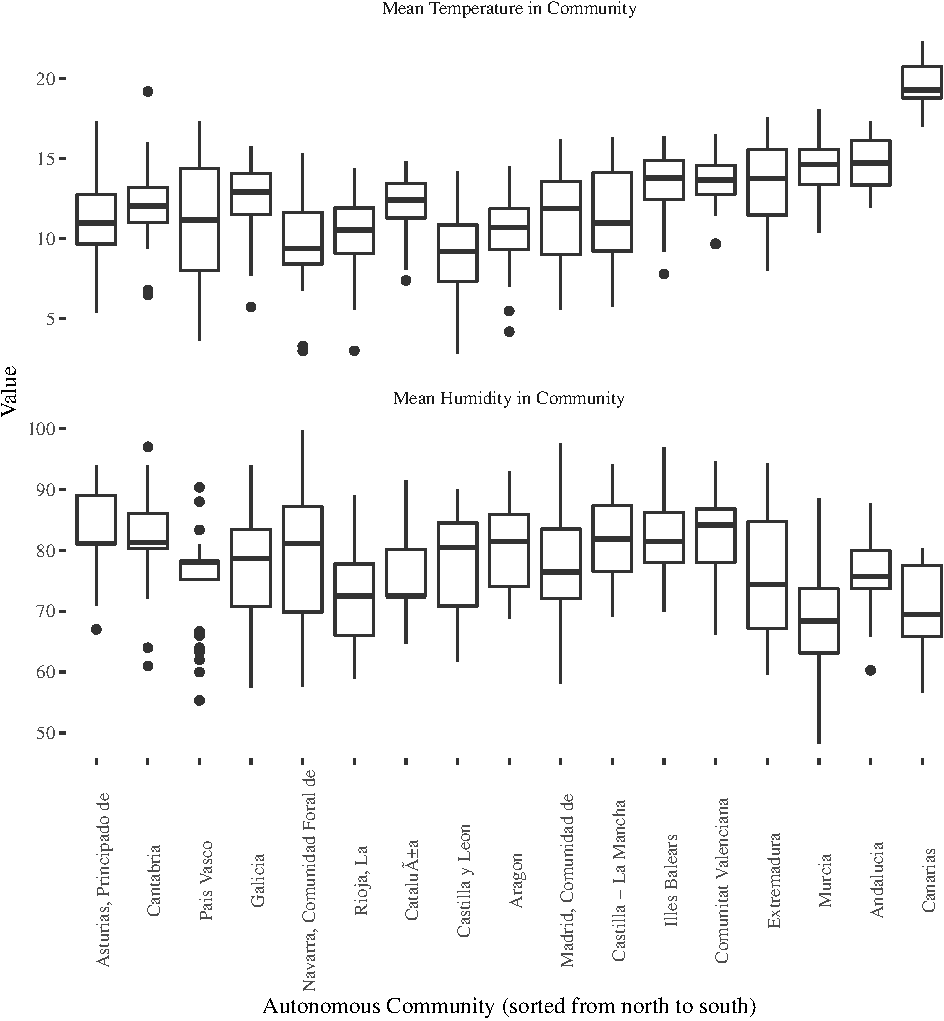
\includegraphics{Environmental-Correlates-of-COVID19-Spain_files/figure-latex/descriptives-temperature-1.pdf}
\caption{\label{fig:descriptives-temperature} Distribution of mean
temperatures and humidities in the Autonomous Communities in Spain
between March 12, 2020 and April 11, 2020. The Autonomous Communities
have been sorted by latitude, with communities to the left being the
northermost, and to the right the southernmost}
\end{figure}

Figure \ref{fig:map-controls} includes three maps that display the
spatial variation of our control variables, namely GDP per capita,
percentage of older adults in province, population density, and presence
of mass transit systems. As seen there, GDP per capita is higher in
Madrid and the northeast part of the country, mainly in Pais Vasco and
Cataluña. Percentage of older adults is somewhat more checkered, with
high values in Madrid and other provinces in the center-west part of the
country, but also in some provinces in the north. Outside of provinces
with major cities (e.g., Madrid; Bizkaia and Gipuzkoa in Pais Vasco;
Pontevedra in Galicia), population density tends to be higher in
provinces along the Mediterranean coast. The final panel in the figure
shows the five provinces in the country that have higher order mass
transit systems (e.g., metro).

\begin{figure}
\centering
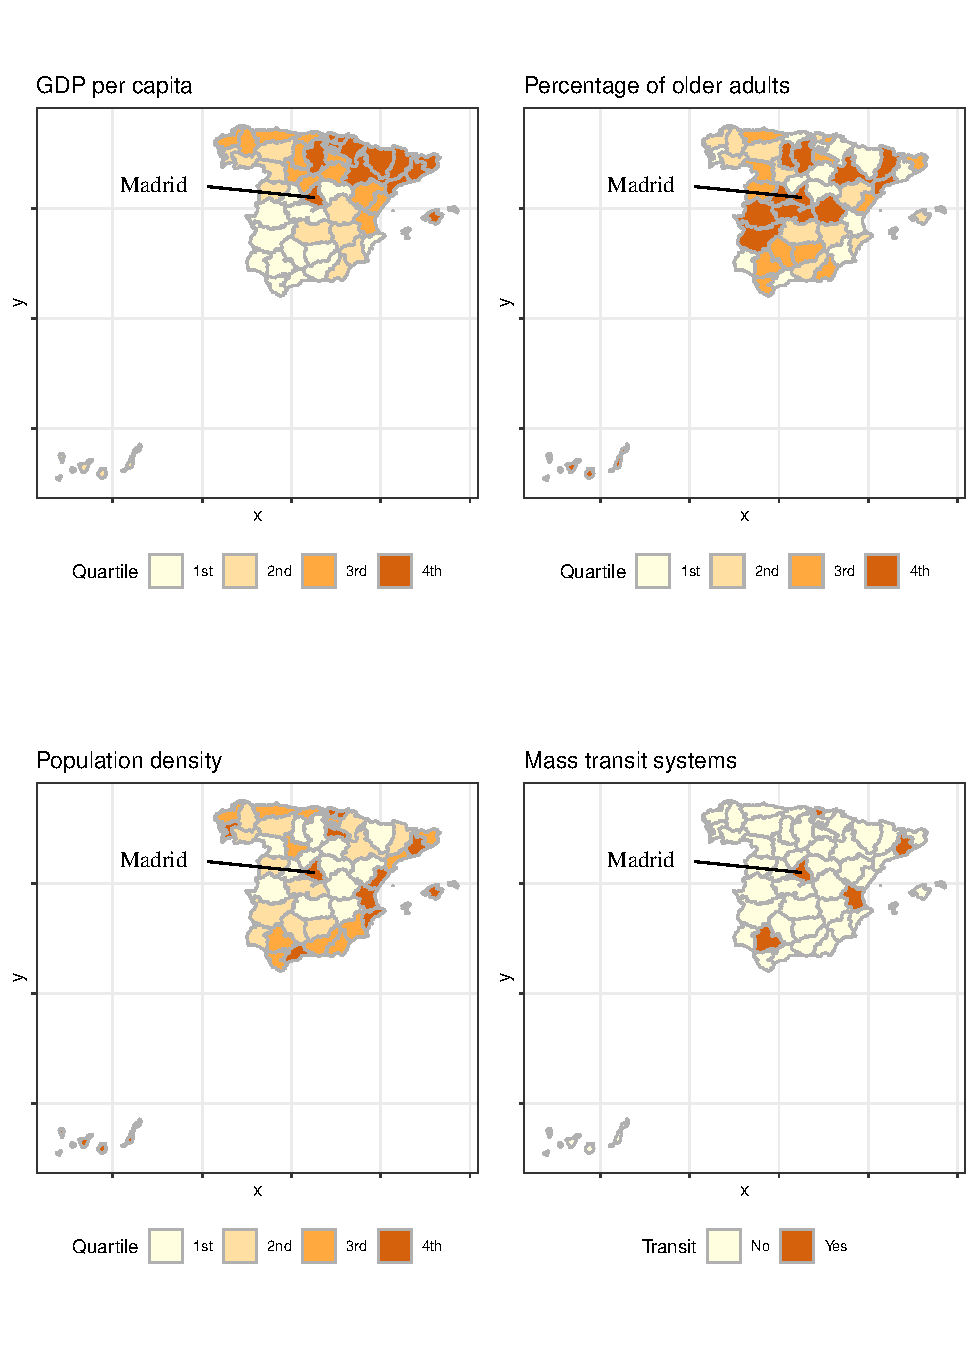
\includegraphics{Environmental-Correlates-of-COVID19-Spain_files/figure-latex/map-controls-1.pdf}
\caption{\label{fig:map-controls}Spatial distribution of control
variables by province}
\end{figure}

Figure \ref{fig:daily-correlations} shows the distribution of daily
simple correlations of incidence of COVID-19 with the independent
variables (with the exception of Transit, which is a categorical
variable). These correlations are calculated after log-transforming all
variables. As previously discussed, the environmental variables have a
temporal lag and were calculated using different time windows.

It can be seen in the figure that temperature (in its three forms) has
the highest simple correlation with incidence of COVID-19. After
temperature, GDP per capita has the highest positive correlation with
the dependent variable. The distribution of these correlations is also
quite tight over the 30-day period of the study. Hours of sunshine tends
to have a moderately high correlation with incidence of COVID-19, but
the distribution of these correlations is more spread, and in some cases
strays into negative values. A similar thing happens with humidity,
which also tends to display more day to day variation in the correlation
with the dependent variable. The percentage of older adults shows a
relatively tight distribution of day-to-day correlations, and is
negative. Population density, in contrast, tends to be negative, but is
relatively spread, and on some days, the simple correlation between
density and incidence of COVID-19 is weakly positive. Overall for the
period under examination, the pairwise correlations between these
variables and incidence are significant at \(p<0.05\), with the
exception of the three Sunshine\_hours variables.

\begin{figure}
\centering
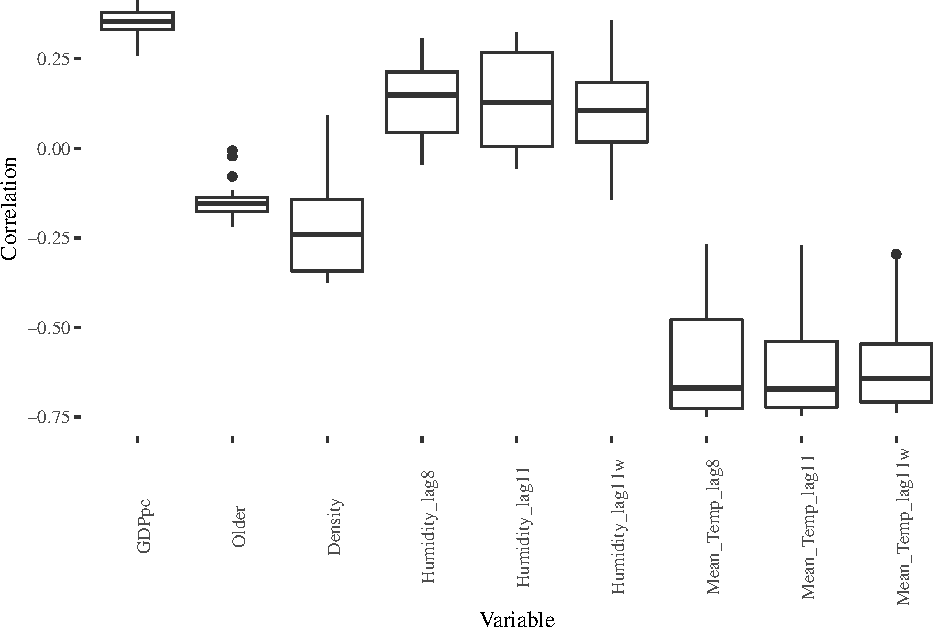
\includegraphics{Environmental-Correlates-of-COVID19-Spain_files/figure-latex/daily-correlations-1.pdf}
\caption{\label{fig:daily-correlations}Distribution of daily
correlations of the independent variables with daily incidence of
COVID-19 (all variables have been log-transformed)}
\end{figure}

\hypertarget{sur-models}{%
\subsection{SUR Models}\label{sur-models}}

Correlation analysis in the preceding section provides some insights
about the potential associations between incidence of COVID-19 and the
various environmental and control variables. In this section we estimate
three spatial SUR models to test the differences between the various
temporal lags and weighting schemes for the environmental variables.
Accordingly, we define three models: Model 1, which is estimated using
the lagged 8-day averages of the environmental variables (\emph{lag8});
Model 2, which is estimated using the lagged 11-day averages of the
environmental variables (\emph{lag11}); and finally, Model 3, which is
estimated using the lagged 11-day \emph{weighted} averages of the
environmental variables (\emph{lag11w}).

To implement the SUR approach, we must define a matrix of spatial
weights \(W\). In this case, we consider neighborhoods based on
adjacency, based on the well-known queen criterion (two provinces are
adjacent if they share a boundary or touch at a vertex). The analysis is
of the coterminous
provinces\footnote{As a check for robustness, we also tested the rook criterion (two provinces are adjacent if they share a boundary, but not if they only touch at a vertex), and included the three islands in the sample. In this case we made an allowance for adjacency between the two islands in the Autonomous Community of Canarias in the Pacific (Las Palmas and Santa Cruz de Tenerife), and assumed that Islas Baleares in the Mediterranean are adjacent to three provinces in Pais Catalans (i.e., Barcelona, Tarragona, and Castello) The results (which can be consulted in the source R markdown document) are robust to the specification of $W$.}.

For estimation, we log-transform the dependent and quantitative
independent variables. The only variable that is not transformed is the
categorical variable for transit systems. A log-log transformation is
appropriate to capture non-linear relationships between variables and
provides a straightforward interpretation of the coefficients as
percentage change. Furthermore, we introduce restrictions so that the
coefficients of two of our control variables are constant over time,
namely GDP per capita and percentage of older adults. We do not see an
\emph{a priori} reason to let those two variables vary across equations,
and the correlation analysis in Figure \ref{fig:daily-correlations} also
suggest little temporal variation. In contrast, we let the spatial
autocorrelation parameter, as well as the parameters of the rest of the
independent variables (including the constant) to vary over
time\footnote{We conducted sensitivity analysis letting all parameters vary over time, and while the results are qualitatively similar, the resulting models are less parsimonious. These results are available in the source R markdown document.}.
This will be useful to detect whether there are behavioral adaptations
at the population level over the course of the period examined. As an
example of behavioral adaptations, the effect of density might weaken
over time, in the measure that the effects of the lockdown are felt: at
full compliance with the lockdown, with people practicing social
avoidance, density might matter less than other factors.

After estimation, we compare the goodness of fit of the three SUR
models. Figure \ref{fig:goodness-of-fit} shows the equation-level
coefficient of determination \(R^2\), one for each time period/day. As
well, the overall coefficient of determination for the system is
reported for each model \(\text{pooled}-R^2\). The general trend is
identical for the three models, with the goodness-of-fit improving over
time and plateuing around a value of \(R^2\) of 0.55. Model 1
(\emph{lag8}) performs somewhat better in the first few equations/days,
when the goodness-of-fit is relatively poor, and then again in the last
few equations/days. Model 3 (\emph{lag11w}), in contrast, does not
perform well towards the end of the study period. The most balanced
model in terms of equation-level goodness-of-fit appears to be Model 1
(\emph{lag8}), and this impression is further supported by a slightly
higher value of the \(\text{pooled}-R^2\). The analysis using a lagged
moving average of the environmental variables is generally in line with
the incubation period reported by Lauer et al.~(2020), although the
results do not support the use of a weighted average. For the remainder
of the paper, we will adopt Model 1 (\emph{lag8}) as our best model. In
the following section we discuss the results of the analysis in more
depth.

\begin{figure}
\centering
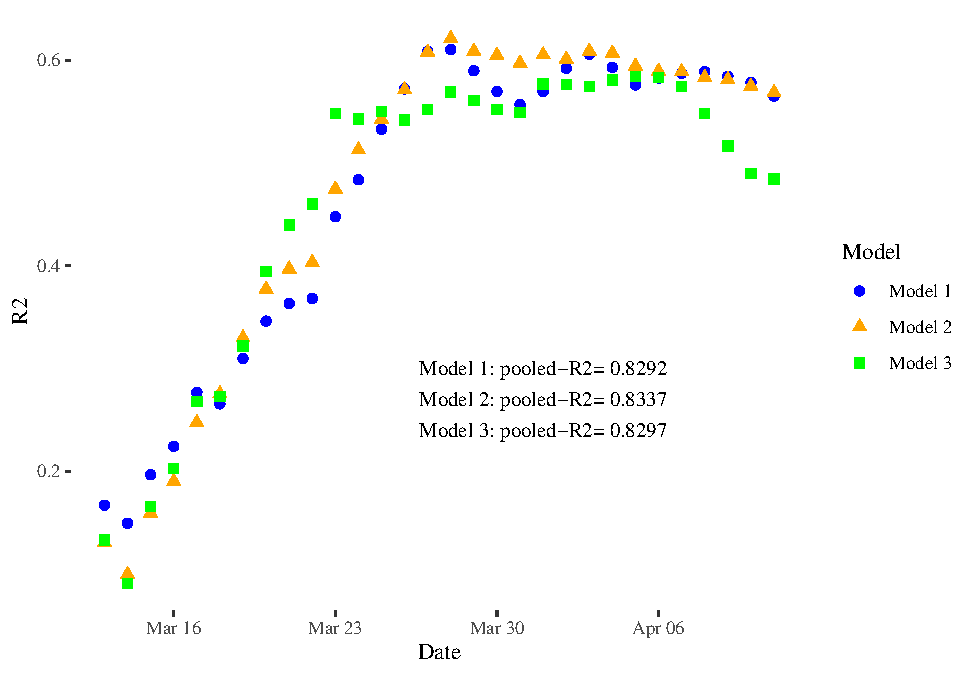
\includegraphics{Environmental-Correlates-of-COVID19-Spain_files/figure-latex/goodness-of-fit-1.pdf}
\caption{\label{fig:goodness-of-fit} Goodness of fit of the SUR systems:
by date and pooled}
\end{figure}

\hypertarget{discussion}{%
\section{Discussion}\label{discussion}}

Table \ref{tab:summary-best-model} presents a summary of the results of
Model 1 (\emph{lag8}). Recall that two coefficients were constrained and
are estimated only for the first equation of the system, and thus are
assumed to be constant over time. These are the coefficients
corresponding to GDP per capita (\(p\leq0.10\)) and percentage of older
adults (\(p\leq0.05\)). The sign of the coefficient for GDP per capita
is positive, which indicates that wealthier regions tend to have a
higher incidence of COVID-19. This is in line with the idea that the
epidemic started earlier in wealthier places due to their connections to
a globalized world. The sign of the coefficient for percentage of older
adults, on the other hand, is negative. As previously discussed, the
level of social contact of older adults even under normal circumstances
tends to be lower than for younger people. As a consequence, places with
larger populations of older adults appear to have a natural level of
social distancing in place. It is important to note that this does not
detract from evidence that older adults are more vulnerable individually
and in institutional settings, where their case mortality rates are
perhaps the highest of all age groups. Instead, this result indicates
that their presence in the community at large tends to depress
transmission of the virus.

Of the two other control variables, the coefficient of population
density is significant at \(p\leq0.05\) in 12, at \(p\leq0.10\) in 3
equations, and not significant in 15. The coefficient for transit is
significant at \(p\leq0.10\) in 20 equations, and of those, significant
at \(p\leq0.05\) in 18 equations. The next four variables are
environmental factors. The coefficient for humidity is significant at
\(p\leq0.19\) in 20 equations, and of those, significant at
\(p\leq0.05\) in 15 equations. Of the environmental variables,
temperature is the only variable that has significant coefficients in
every equation at \(p\leq0.05\). Finally, sunshine has significant
coefficients at \(p\leq0.05\) in 24 equations.

\begin{table}

\caption{\label{tab:summary-best-model}\label{tab:summary-best-model}Summary of estimation results of best model (lag11: lagged 11-day moving average)}
\centering
\resizebox{\linewidth}{!}{
\begin{tabular}[t]{lrrrrrrl}
\toprule
\multicolumn{1}{c}{ } & \multicolumn{3}{c}{Estimates} & \multicolumn{3}{c}{Significance} & \multicolumn{1}{c}{ } \\
\cmidrule(l{3pt}r{3pt}){2-4} \cmidrule(l{3pt}r{3pt}){5-7}
Variable & Min & Mean & Max & p > 0.10 & 0.10 <= p < 0.05 & p <= 0.05 & Note\\
\midrule
\rowcolor{gray!6}  Intercept & 6.172 & 9.441 & 14.071 & 0 & 0 & 30 & Non-constrained\\
log(GDPpc) & 0.449 & 0.449 & 0.449 & 0 & 1 & 0 & Constrained\\
\rowcolor{gray!6}  log(Older) & -0.676 & -0.676 & -0.676 & 0 & 0 & 1 & Constrained\\
log(Density) & -0.212 & -0.105 & 0.143 & 15 & 3 & 12 & Non-constrained\\
\rowcolor{gray!6}  Transit & 0.341 & 0.528 & 0.606 & 10 & 2 & 18 & Non-constrained\\
\addlinespace
log(Humidity) & -1.935 & -0.435 & 0.054 & 11 & 4 & 15 & Non-constrained\\
\rowcolor{gray!6}  log(Temperature) & -1.904 & -1.236 & -0.817 & 0 & 0 & 30 & Non-constrained\\
log(Sunshine) & -0.187 & 0.099 & 0.189 & 6 & 0 & 24 & Non-constrained\\
\rowcolor{gray!6}  Spatially lagged y (rho) & 0.014 & 0.154 & 0.348 & 14 & 3 & 13 & Non-constrained\\
\bottomrule
\multicolumn{8}{l}{\textit{Note: }}\\
\multicolumn{8}{l}{Significance: This is the number of coefficients with p-values as indicated}\\
\multicolumn{8}{l}{Non-constrained: coefficient was allowed to vary across equations}\\
\multicolumn{8}{l}{Constrained: coefficient as constant across equations}\\
\end{tabular}}
\end{table}

To better understand the results, we proceed to plot the coefficients in
their temporal sequence. At this point it is worth recalling that the
state of emergency went into effect on March 14. In the following
figures, the periods of time indicated in yellow starting on March 14
correspond to the state of emergency, with only essential travel and
selected industrial activities allowed; the period of time in orange was
the stricter lockdown when only essential travel was allowed.

We begin our discussion with the evolution of the spatial
autocorrelation coefficient (\(\rho\)) in Figure
\ref{fig:results-time-1} (left panel). We notice that the magnitude of
the spatial autocorrelation coefficient \(\rho\) declines over the
period under analysis, and is not significant for some days. This is an
interesting result: immediately prior to the declaration of the state of
emergency, there appears to have been a strong inter-provincial
contagion effect. Keeping in mind that the incubation period ranges
between 2 and 12 days with a median of 5, it is reasonable to expect
that the effect of the lockdown will be observed with some delay.
Indeed, as seen in the figure, the autocorrelation coefficient remains
high for several days, then begins to decline around March 23, and
continues to weaken over time. At the end of the period under
examination, the strength of this effect is much diminished and we would
expect that under full compliance with strict lockdown conditions
(meaning no inter-provincial mobility) the spatial contagion effect
would be zero - as seems to be the case.

The intercept (right panel in Figure \ref{fig:results-time-1}) is
indicative of the variation of the incidence of COVID-19, other things
being equal. Here we see that at the incidence declines somewhat
immediately after the state of emergency, only to begin increasing again
over time. Then, the incidence declines again after the stricter
lockdown and rebounds to a lower level by April 11.

\begin{figure}
\centering
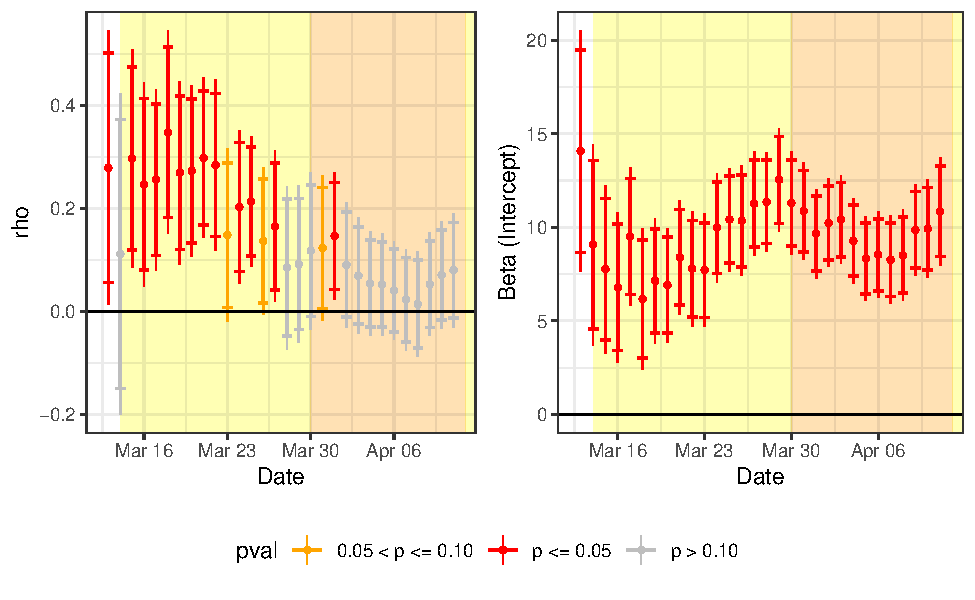
\includegraphics{Environmental-Correlates-of-COVID19-Spain_files/figure-latex/results-time-1-1.pdf}
\caption{\label{fig:results-time-1}Temporal evolution of the spatial
autocorrelation coefficient (rho) and the intercept of the model; dots
are the point estimates and vertical lines are 95\% confidence
intervals. In yellow is the period after the declaration of the state of
emergency, and in orange is the period when only essential activities
were allowed.}
\end{figure}

Figure \ref{fig:beta-controls-time} shows the temporal evolution of the
coefficients for the two control variables that were not fixed over
time, i.e., \(\log(Density)\) (left panel) and \(Transit\) (right
panel).

In Section \ref{background} we had anticipated a positive sign for the
coefficient of density, and indeed, at the beginning of the period the
coefficient is positive, albeit not significant, and then remains mostly
non-significant for the earlier part of the lockdown. We are somewhat
surprised by the way this coefficient turns significant \emph{and}
negative in the later part of the lockdown, after April 1st. This
effect, we surmise, is the result of risk compensation, a situation
where people adapt their behavior according to the \emph{perceived}
level of risk, becoming more careful when the perceived risk is higher
and viceversa (e.g., Noland, 1995; Phillips et al., 2011; Richens et
al., 2000). Consequently, residents in high density regions may perceive
the risk of infection as being higher, and adapt their behavior
accordingly - while the opposite may be true of residents in low density
regions. The coefficient for Transit is positive, as expected, but with
very wide confidence intervals, and in fact not significant in the
earlier part of the period.

\begin{figure}
\centering
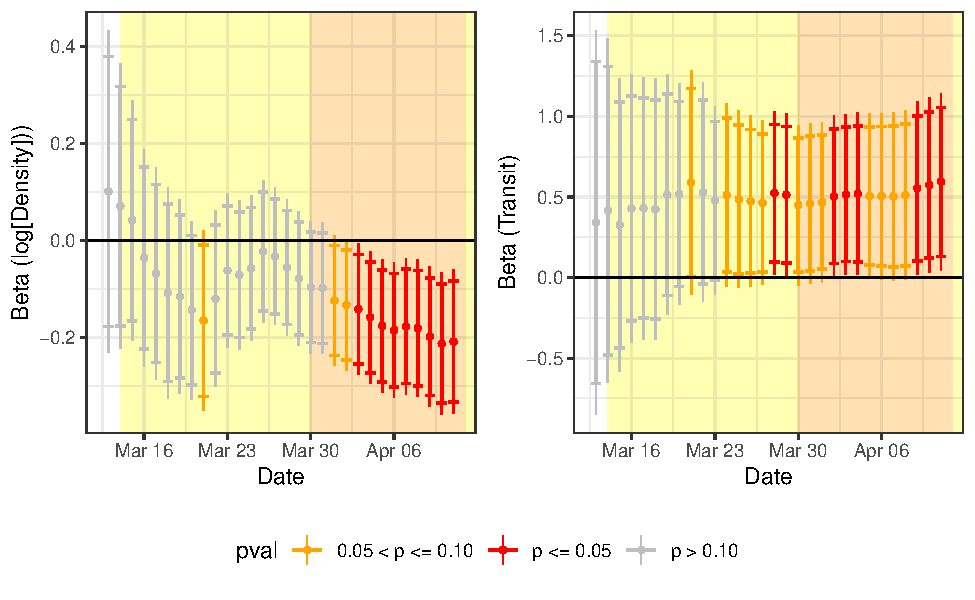
\includegraphics{Environmental-Correlates-of-COVID19-Spain_files/figure-latex/beta-controls-time-1.pdf}
\caption{\label{fig:beta-controls-time}Temporal evolution of coefficient
for the control variables; dots are the point estimates and vertical
lines are 95\% confidence intervals. In yellow is the period after the
declaration of the state of emergency, and in orange is the period when
only essential activities were allowed.}
\end{figure}

The evolution of the coefficients for the three environmental variables
is shown in Figure \ref{fig:beta-environmental-time}. Despite a mostly
positive simple correlation with incidence (see Figure
\ref{fig:daily-correlations}) once that we control for other factors,
humidity has a negative association with incidence of COVID-19 in Spain
(top-right panel). This is in line with the literature that describes
the lower viability and transmission of different viruses at higher
levels of humidity. The coefficients for temperature (top-right panel)
are consistently negative and this variable is, besides the intercept,
the only one with significant coefficients in all equations. The range
of variation of this coefficient during the period examined is
approximately between -1 and -2, although it is important to recall that
these values should not be interpreted directly as effects; more on this
below. Finally the plot for the coefficients associated with hours of
sunshine (bottom panel) is more ambiguous: prior to the lockdown, the
coefficient was negative, but not significant. However, five days into
the lockdown, the coefficient becomes significant and \emph{positive}.
This result stands in contrast to previous findings regarding influenza,
where more hours of sunlight reduced the strength and duration of
epidemic durations (Yu et al., 2013). A difference with previous studies
is the temporal scale of the analysis: where Yu et al.~(2013) use
monthly averages, we use daily data for a much shorter period of time.
The positive sign of sunshine may well be another instance of behavioral
adaptations, whereby compliance with lockdown orders weakens on sunny
days.

\begin{figure}
\centering
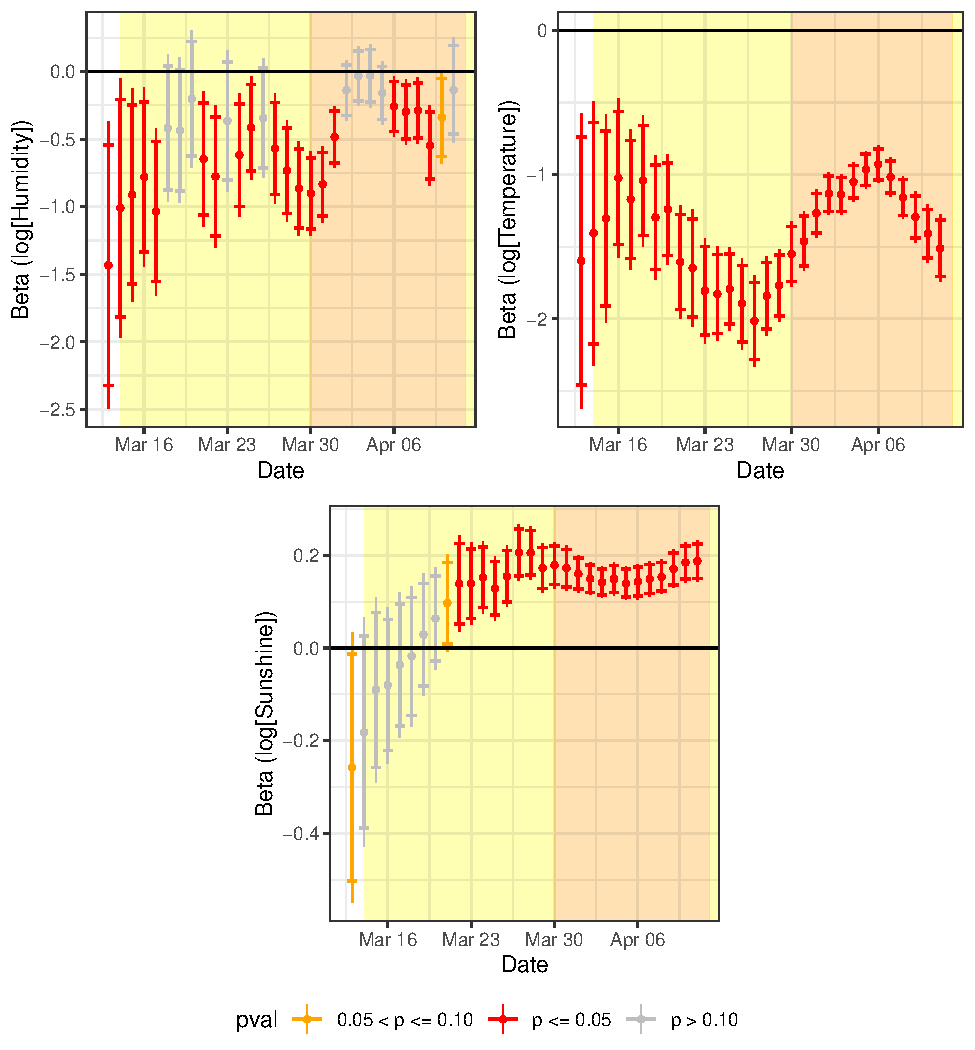
\includegraphics{Environmental-Correlates-of-COVID19-Spain_files/figure-latex/beta-environmental-time-1.pdf}
\caption{\label{fig:beta-environmental-time}Temporal evolution of
coefficient for the environmental variables; dots are the point
estimates and vertical lines are 95\% confidence intervals. In yellow is
the period after the declaration of the state of emergency, and in
orange is the period when only essential activities were allowed.}
\end{figure}

The preceding discussion helps to establish the inferential
contributions of the analysis, and indicate which variables display
significant statistical associations with incidence of COVID-19. The
remaining question is, what are the implications.

As discussed in Section \ref{methods} the effect of a variable is not
clear from its coefficient alone, since a change to a variable in a
province influences, via the contagion effect, its neighbors. For this
reason, the appropriate way to estimate the effects is to calculate both
the own effect and the effect due to contagion, or in other words the
direct and indirect effects, respectively. The total effect is the sum
of the two. A summary of the effects appears in Table
\ref{tab:summary-impacts-best-model}. All effects in the table are
interpreted as percentage change in the incidence of COVID-19 as a
consequence of a one percent change in the variable. The exception to
this is Transit (which was not log-transformed). This variable instead
represents the percentage change in incidence between provinces without
and with mass transit systems.

Two variables had temporally constrained coefficients. The estimated
effect of GDP per capita is to increase the incidence of COVID-19 by
0.449\% for each percent increase of this variable (in €1,000s). In our
view, this is a measure of inertia, as provinces with higher GDP per
capita where among the first to see exponential growth in the pandemic.
Percentage of older adults has a negative effect, and each percent
increase in this variable is associated with a relatively small
reduction of the incidence of approximately 0.67\%.

The temporal variation of the effects for the rest of the variables is
shown in Figure \ref{fig:plot-impacts}. The largest positive direct
effect is Transit, and the largest direct negative effects are
temperature and humidity. The direct effects of these variables are as
follows: for each percent point increase in temperature, there is
between a 1\% and 2\% reduction in the incidence of the disease. This
effect is compounded via contagion, as seen in the central panel in the
figure, and the indirect effect can further reduce the incidence by up
to 0.75\%. The effect of humidity is also to reduce the incidence: each
percent point of increase in humidity is associated with a reduction of
up to 2\% in incidence. With the addition of the indirect effect, the
total effect of a 1\% increase in humidity is to reduce incidence by up
to 3\%. As seen in the figure, the indirect (i.e., contagion) effects
are stronger at the before and at the beginning of the lockdown period.
Nonetheless, by the end of the period under study, the indirect effects
have weakened considerably.

What do these effects mean? Under a situation of lockdown,
inter-regional contagion is reduced, as expected, and the total effects
of the variables tend towards their direct effects. In the first few
days covered by our analysis the total effect of all variables is
greater due to the spatial contagion effect. Contagion makes analysis
and intervention more complex: the contagion effect essentially acts
like a multiplier, whereby developments in each province spill over to
their neighbors. Once the contagion effect has been tamed, each province
can be ``treated'' independently from its neighbors.

It is important, before concluding our discussion, to highlight some
limitations of this study.

First, the analysis was conducted mostly under a situation of lockdown,
and therefore, besides first days of the period examined, one must
exercise caution when trying to extrapolate the findings to a situations
without lockdown. Secondly, it is well known that there is in many
countries substantial underreporting of cases of COVID-19 due to limited
testing. In this case we do not suspect systematic provincial bias in
reporting, and as long as the underreporting is consistent across units
of analysis, we do not expect biased results; it is still important,
however, to remain aware that the number of true cases is likely higher.
Finally, we defined neighborhoods based on adjacency. It would be
interesting to compare adjacency to other connectivity criteria, for
instance based on domestic transportation instrastructure and services.
We flag this as a matter for future research.

\begin{table}

\caption{\label{tab:summary-impacts-best-model}\label{tab:summary-impacts-best-model}Summary of direct, indirect, and total effects according to best model (lag8: lagged 8-day moving average)}
\centering
\begin{tabular}[t]{lrrrl}
\toprule
Variable & Min & Mean & Max & Note\\
\midrule
\rowcolor{gray!6}  \addlinespace[0.3em]
\multicolumn{5}{l}{\textbf{Direct Effects}}\\
\hspace{1em}log(GDPpc) & 0.457 & 0.457 & 0.457 & Constrained\\
\hspace{1em}log(Older) & -0.688 & -0.688 & -0.688 & Constrained\\
\rowcolor{gray!6}  \hspace{1em}log(Density) & -0.213 & -0.106 & 0.145 & Non-constrained\\
\hspace{1em}Transit & 0.349 & 0.532 & 0.608 & Non-constrained\\
\rowcolor{gray!6}  \hspace{1em}log(Humidity) & -1.971 & -0.440 & 0.054 & Non-constrained\\
\hspace{1em}log(Temperature) & -1.939 & -1.245 & -0.825 & Non-constrained\\
\rowcolor{gray!6}  \hspace{1em}log(Sunshine) & -0.191 & 0.099 & 0.190 & Non-constrained\\
\addlinespace[0.3em]
\multicolumn{5}{l}{\textbf{Indirect Effects}}\\
\hspace{1em}log(GDPpc) & 0.165 & 0.165 & 0.165 & Constrained\\
\rowcolor{gray!6}  \hspace{1em}log(Older) & -0.249 & -0.249 & -0.249 & Constrained\\
\hspace{1em}log(Density) & -0.075 & -0.015 & 0.052 & Non-constrained\\
\rowcolor{gray!6}  \hspace{1em}Transit & 0.008 & 0.097 & 0.240 & Non-constrained\\
\hspace{1em}log(Humidity) & -0.712 & -0.104 & 0.001 & Non-constrained\\
\rowcolor{gray!6}  \hspace{1em}log(Temperature) & -0.700 & -0.238 & -0.013 & Non-constrained\\
\hspace{1em}log(Sunshine) & -0.069 & 0.017 & 0.063 & Non-constrained\\
\rowcolor{gray!6}  \addlinespace[0.3em]
\multicolumn{5}{l}{\textbf{Total Effects}}\\
\hspace{1em}log(GDPpc) & 0.622 & 0.622 & 0.622 & Constrained\\
\hspace{1em}log(Older) & -0.937 & -0.937 & -0.937 & Constrained\\
\rowcolor{gray!6}  \hspace{1em}log(Density) & -0.265 & -0.121 & 0.198 & Non-constrained\\
\hspace{1em}Transit & 0.466 & 0.629 & 0.847 & Non-constrained\\
\rowcolor{gray!6}  \hspace{1em}log(Humidity) & -2.683 & -0.543 & 0.055 & Non-constrained\\
\hspace{1em}log(Temperature) & -2.640 & -1.483 & -0.870 & Non-constrained\\
\rowcolor{gray!6}  \hspace{1em}log(Sunshine) & -0.259 & 0.116 & 0.235 & Non-constrained\\
\bottomrule
\multicolumn{5}{l}{\textit{Note: }}\\
\multicolumn{5}{l}{Non-constrained: coefficient was allowed to vary across equations}\\
\multicolumn{5}{l}{Constrained: coefficient as constant across equations}\\
\end{tabular}
\end{table}

\begin{figure}
\centering
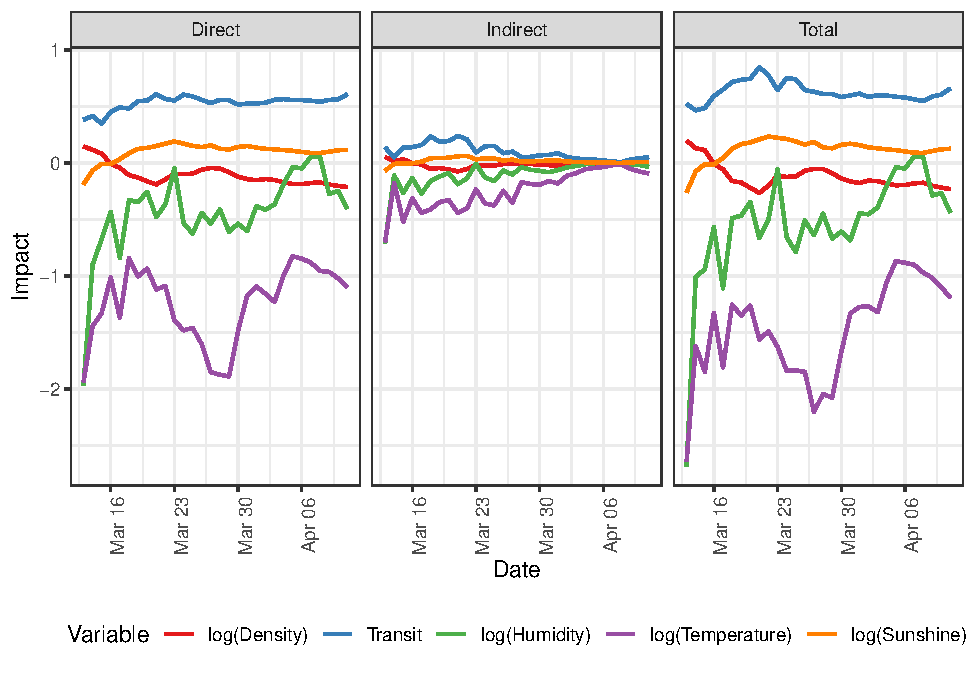
\includegraphics{Environmental-Correlates-of-COVID19-Spain_files/figure-latex/plot-impacts-1.pdf}
\caption{\label{fig:plot-impacts}Temporal evolution of direct, indirect,
and total effects by date.}
\end{figure}

\hypertarget{conclusion}{%
\section{Concluding Remarks}\label{conclusion}}

In this paper we presented a spatio-temporal analysis of incidence of
COVID-19 in Spain. The analysis covers a 30-day period that begins
immediately before the state of emergency was declared in the country.
The focus of the research has been on the environmental correlates of
incidence of the disease. There is a need for more empirical evidence,
as policy makers, public health practitioners, and the public begin
planning for the months ahead at this early stage of the pandemic.

Our results offer strong support for the hypothesis that incidence of
COVID-19 at the population level is lower at higher temperatures and
levels of humidity: the estimated effect is a reduction in the
neighborhood of 3\% percent in incidence per each 1\% increase in
temperature, and a 3\% reduction in incidence per 1\% increase in
humidity \emph{under conditions of contagion}. These reductions are
lower when contagion has ceased (i.e., due to lockdown conditions). The
question here seems to be whether these environmental variables can
yield a bigger reduction of \emph{more} cases, or a smaller reduction of
\emph{fewer} cases.

Our control variables also offer some interesting insights. In
particular, there is evidence of behavioral adaptations during lockdown
in the form of risk compensation (density) and compliance with the
lockdown (sunshine). These results offer a cautionary tale with regards
to the effectiveness of the lockdown in more dense areas, and also the
implications for compliance with stay-at-home orders as the northern
hemisphere moves towards summer and more hours of sunshine during the
day. If risk compensation is a factor, then efforts should be made to
reduce or eliminate risk compensation in less densely populated regions.

A key aspect of the analysis using spatial SUR models is that we were
able to model incidence of COVID-19 as an interregional contagion
process. Here, we find that the strength of the contagion effect was
dramatically reduced by the lockdown.

Needless to say, the analysis presented here is at the level of
population health. For this reason, the analysis does not make any
claims with respect to the effect of ultraviolet light on the virus, but
rather about transmission of the virus in the population. For example,
the analysis does not imply that the virus moves less effectively in
places where more people live in close proximity to each other, but
rather that humans are more contagious when they feel safe in less dense
regions. Similarly, more sunshine does not mean that the virus thrives,
but rather that humans are more contagious to each other when their
behavior adapts to this environmental condition.

Some directions for future research include investigating other
modelling frameworks, such as geographically and temporally weighted
regression and/or space-time conditional autoregressive models. In
addition, the environmental variables examined here relate to
meteorological conditions only, and did not include other environmental
factors that may incide in the transmission of the virus, such as
pollution. These other factors should be incorporated in future studies.

\hypertarget{acknowledgments}{%
\section*{Acknowledgments}\label{acknowledgments}}
\addcontentsline{toc}{section}{Acknowledgments}

Add acknowledgments as appropriate in final draft.

The following \texttt{R} packages were used in the course of this
investigation and the authors wish to acknowledge their developers:
\texttt{aemet} (Rodriguez-Sanchez et al., 2018), \texttt{ggthemes}
(Arnold, 2019), \texttt{gridExtra} (Auguie, 2017), \texttt{kableExtra}
(Zhu, 2019), \texttt{knitr} (Xie, 2015, 2014), \texttt{lubridate}
(Grolemund and Wickham, 2011), \texttt{plm} (Millo, 2017),
\texttt{rticles} (Allaire et al., 2020), \texttt{sf} (Pebesma, 2018),
\texttt{spdep} (Bivand et al., 2013), spsur (Angulo et al., 2020)
\texttt{tidyverse} (Wickham et al., 2019), \texttt{units} (Pebesma et
al., 2016).

\hypertarget{references}{%
\section*{References}\label{references}}
\addcontentsline{toc}{section}{References}

\hypertarget{refs}{}
\leavevmode\hypertarget{ref-Allaire2020}{}%
Allaire, J., Xie, Y., R Foundation, Wickham, H., Journal of Statistical
Software, Vaidyanathan, R., Association for Computing Machinery,
Boettiger, C., Elsevier, Broman, K., Mueller, K., Quast, B., Pruim, R.,
Marwick, B., Wickham, C., Keyes, O., Yu, M., Emaasit, D., Onkelinx, T.,
Gasparini, A., Desautels, M.-A., Leutnant, D., MDPI, Taylor and Francis,
Ögreden, O., Hance, D., Nüst, D., Uvesten, P., Campitelli, E.,
Muschelli, J., Kamvar, Z.N., Ross, N., Cannoodt, R., Luguern, D.,
Kaplan, D.M., 2020. Rticles: Article formats for r markdown.

\leavevmode\hypertarget{ref-Angulo2020spsur}{}%
Angulo, A., Lopez, F.A., Minguez, R., Mur, J., 2020. Spsur: Spatial
seemingly unrelated regression models.

\leavevmode\hypertarget{ref-Anselin1988spatial}{}%
Anselin, L., 1988. Spatial econometrics: Methods and models, Studies in
operational regional science. Kluwer Academic Publishers, Dordrecht.

\leavevmode\hypertarget{ref-Anselin2016estimation}{}%
Anselin, L., 2016. Estimation and testing in the spatial seemingly
unrelated regression (sur). Geoda Center for Geospatial Analysis;
Computation, Arizona State University. Working Paper 2016-01.

\leavevmode\hypertarget{ref-Araujo2020spread}{}%
Araujo, M.B., Naimi, B., 2020. Spread of sars-cov-2 coronavirus likely
to be constrained by climate. medRxiv.

\leavevmode\hypertarget{ref-Arnold2019}{}%
Arnold, J.B., 2019. Ggthemes: Extra themes, scales and geoms for
'ggplot2'.

\leavevmode\hypertarget{ref-Auguie2017gridextra}{}%
Auguie, B., 2017. GridExtra: Miscellaneous functions for "grid"
graphics.

\leavevmode\hypertarget{ref-deangel2020weathering}{}%
Ángel Solá, D.E. de, Wang, L., Vázquez, M., Lázaro, P.A.M., 2020.
Weathering the pandemic: How the caribbean basin can use viral and
environmental patterns to predict, prepare and respond to covid‐19.
Journal of Medical Virology.

\leavevmode\hypertarget{ref-Bivand2013}{}%
Bivand, R.S., Pebesma, E., Gomez-Rubio, V., 2013. Applied spatial data
analysis with R, second edition. Springer, NY.

\leavevmode\hypertarget{ref-Cao2010spatio}{}%
Cao, Z., Zeng, D., Zheng, X., Wang, Q., Wang, F., Wang, J., Wang, X.,
2010. Spatio-temporal evolution of beijing 2003 sars epidemic. Science
China Earth Sciences 53, 1017--1028.
doi:\href{https://doi.org/10.1007/s11430-010-0043-x}{10.1007/s11430-010-0043-x}

\leavevmode\hypertarget{ref-Casanova2010effects}{}%
Casanova, L.M., Jeon, S., Rutala, W.A., Weber, D.J., Sobsey, M.D., 2010.
Effects of air temperature and relative humidity on coronavirus survival
on surfaces. Appl. Environ. Microbiol. 76, 2712--2717.

\leavevmode\hypertarget{ref-Chan2011effects}{}%
Chan, K., Peiris, J., Lam, S., Poon, L., Yuen, K., Seto, W., 2011. The
effects of temperature and relative humidity on the viability of the
sars coronavirus. Advances in virology 2011.

\leavevmode\hypertarget{ref-Cliff1998detecting}{}%
Cliff, A., Haggett, P., Smallman-Raynor, M., 1998. Detecting
space---time patterns in geocoded disease data. Cholera in london, 1854
measles in the united states, 1962--95, in: Geomed'97. Springer, pp.
13--42.

\leavevmode\hypertarget{ref-Coelho2020exponential}{}%
Coelho, M.T.P., Rodrigues, J.F.M., Medina, A.M., Scalco, P., Terribile,
L.C., Vilela, B., Diniz-Filho, J.A.F., Dobrovolski, R., 2020.
Exponential phase of covid19 expansion is not driven by climate at
global scale. medRxiv.

\leavevmode\hypertarget{ref-Desjardins2020rapid}{}%
Desjardins, M., Hohl, A., Delmelle, E., 2020. Rapid surveillance of
covid-19 in the united states using a prospective space-time scan
statistic: Detecting and evaluating emerging clusters. Applied Geography
102202.

\leavevmode\hypertarget{ref-Elhorst2014spatial}{}%
Elhorst, J.P., 2014. Spatial econometrics: From cross-sectional data to
spatial panels. Springer.

\leavevmode\hypertarget{ref-Fernandes2020economic}{}%
Fernandes, N., 2020. Economic effects of coronavirus outbreak (covid-19)
on the world economy. Available at SSRN 3557504.

\leavevmode\hypertarget{ref-Golgher2016interpret}{}%
Golgher, A.B., Voss, P.R., 2016. How to interpret the coefficients of
spatial models: Spillovers, direct and indirect effects. Spatial
Demography 4, 175--205.

\leavevmode\hypertarget{ref-Gong2020balance}{}%
Gong, B., Zhang, S., Yuan, L., Chen, K.Z., 2020. A balance act:
Minimizing economic loss while controlling novel coronavirus pneumonia.
Journal of Chinese Governance 1--20.

\leavevmode\hypertarget{ref-Greene2003econometric}{}%
Greene, W.H., 2003. Econometric analysis. Pearson Education India.

\leavevmode\hypertarget{ref-Grolemund2011dates}{}%
Grolemund, G., Wickham, H., 2011. Dates and times made easy with
lubridate. Journal of Statistical Software 40, 1--25.

\leavevmode\hypertarget{ref-Hallet2002regional}{}%
Hallet, M., 2002. Regional specialisation and concentration in the eu,
in: Regional Convergence in the European Union. Springer, pp. 53--76.

\leavevmode\hypertarget{ref-Harbert2020spatial}{}%
Harbert, R.S., Cunningham, S.W., Tessler, M., 2020. Spatial modeling
cannot currently differentiate sars-cov-2 coronavirus and human
distributions on the basis of climate in the united states. medRxiv.

\leavevmode\hypertarget{ref-Hu2013scaling}{}%
Hu, H., Nigmatulina, K., Eckhoff, P., 2013. The scaling of contact rates
with population density for the infectious disease models. Mathematical
Biosciences 244, 125--134.
doi:\href{https://doi.org/https://doi.org/10.1016/j.mbs.2013.04.013}{https://doi.org/10.1016/j.mbs.2013.04.013}

\leavevmode\hypertarget{ref-Jaakkola2014decline}{}%
Jaakkola, K., Saukkoriipi, A., Jokelainen, J., Juvonen, R., Kauppila,
J., Vainio, O., Ziegler, T., Rönkkö, E., Jaakkola, J.J., Ikäheimo, T.M.,
2014. Decline in temperature and humidity increases the occurrence of
influenza in cold climate. Environmental Health 13, 22.

\leavevmode\hypertarget{ref-Jones2008global}{}%
Jones, K.E., Patel, N.G., Levy, M.A., Storeygard, A., Balk, D.,
Gittleman, J.L., Daszak, P., 2008. Global trends in emerging infectious
diseases. Nature 451, 990--993.
doi:\href{https://doi.org/10.1038/nature06536}{10.1038/nature06536}

\leavevmode\hypertarget{ref-Kissler2020projecting}{}%
Kissler, S.M., Tedijanto, C., Goldstein, E., Grad, Y.H., Lipsitch, M.,
2020. Projecting the transmission dynamics of sars-cov-2 through the
postpandemic period. Science eabb5793.
doi:\href{https://doi.org/10.1126/science.abb5793}{10.1126/science.abb5793}

\leavevmode\hypertarget{ref-Kudo2019low}{}%
Kudo, E., Song, E., Yockey, L.J., Rakib, T., Wong, P.W., Homer, R.J.,
Iwasaki, A., 2019. Low ambient humidity impairs barrier function and
innate resistance against influenza infection. Proceedings of the
National Academy of Sciences 116, 10905--10910.

\leavevmode\hypertarget{ref-Lancastle2020impact}{}%
Lancastle, N.M., 2020. Is the impact of social distancing on coronavirus
growth rates effective across different settings? A non-parametric and
local regression approach to test and compare the growth rate. medRxiv.

\leavevmode\hypertarget{ref-Lauer2020incubation}{}%
Lauer, S.A., Grantz, K.H., Bi, Q., Jones, F.K., Zheng, Q., Meredith,
H.R., Azman, A.S., Reich, N.G., Lessler, J., 2020. The incubation period
of coronavirus disease 2019 (covid-19) from publicly reported confirmed
cases: Estimation and application. Annals of Internal Medicine.
doi:\href{https://doi.org/10.7326/m20-0504}{10.7326/m20-0504}

\leavevmode\hypertarget{ref-Lauridsen2010spatiotemporal}{}%
Lauridsen, J., Bech, M., López, F., Maté, M., 2010. A spatiotemporal
analysis of public pharmaceutical expenditure. The Annals of Regional
Science 44, 299--314.

\leavevmode\hypertarget{ref-Legallo2006evaluating}{}%
Le Gallo, J., Dall'Erba, S., 2006. Evaluating the temporal and spatial
heterogeneity of the european convergence process, 1980--1999. Journal
of Regional Science 46, 269--288.

\leavevmode\hypertarget{ref-LeSage2009introduction}{}%
LeSage, J., Pace, R.K., 2009. Introduction to spatial econometrics.
Chapman; Hall/CRC.

\leavevmode\hypertarget{ref-Lewnard2020scientific}{}%
Lewnard, J.A., Lo, N.C., 2020. Scientific and ethical basis for
social-distancing interventions against covid-19. The Lancet. Infectious
diseases S1473--3099(20)30190--0.
doi:\href{https://doi.org/10.1016/S1473-3099(20)30190-0}{10.1016/S1473-3099(20)30190-0}

\leavevmode\hypertarget{ref-Lopez2017spatial}{}%
López, F.A., Martínez-Ortiz, P.J., Cegarra-Navarro, J.-G., 2017. Spatial
spillovers in public expenditure on a municipal level in spain. The
Annals of Regional Science 58, 39--65.

\leavevmode\hypertarget{ref-Lopez2014spatial}{}%
López, F.A., Mur, J., Angulo, A., 2014. Spatial model selection
strategies in a sur framework. The case of regional productivity in eu.
The Annals of Regional Science 53, 197--220.

\leavevmode\hypertarget{ref-Luo2020how}{}%
Luo, S., Tsang, K.P., 2020. How much of china and world gdp has the
coronavirus reduced? Available at SSRN 3543760.

\leavevmode\hypertarget{ref-Makinen2009cold}{}%
Mäkainen, T.M., Juvonen, R., Jokelainen, J., Harju, T.H., Peitso, A.,
Bloigu, A., Silvennoinen-Kassinen, S., Leinonen, M., Hassi, J., 2009.
Cold temperature and low humidity are associated with increased
occurrence of respiratory tract infections. Respiratory medicine 103,
456--462.

\leavevmode\hypertarget{ref-Meijers2008strategic}{}%
Meijers, E., Hoekstra, J., Aguado, R., 2008. Strategic planning for city
networks: The emergence of a basque global city? International Planning
Studies 13, 239--259.
doi:\href{https://doi.org/10.1080/13563470802521440}{10.1080/13563470802521440}

\leavevmode\hypertarget{ref-Meng2005understanding}{}%
Meng, B., Wang, J., Liu, J., Wu, J., Zhong, E., 2005. Understanding the
spatial diffusion process of severe acute respiratory syndrome in
beijing. Public Health 119, 1080--1087.
doi:\href{https://doi.org/https://doi.org/10.1016/j.puhe.2005.02.003}{https://doi.org/10.1016/j.puhe.2005.02.003}

\leavevmode\hypertarget{ref-Millo2017robust}{}%
Millo, G., 2017. Robust standard error estimators for panel models: A
unifying approach. Journal of Statistical Software 82, 1--27.
doi:\href{https://doi.org/10.18637/jss.v082.i03}{10.18637/jss.v082.i03}

\leavevmode\hypertarget{ref-Minguez2019}{}%
Mínguez, R., López, F., Mur, J., 2019. ML versus iv estimates of spatial
sur models: Evidence from the case of airbnb in madrid urban area. The
Annals of Regional Science 1--35.

\leavevmode\hypertarget{ref-Morency2011distance}{}%
Morency, C., Páez, A., Roorda, M.J., Mercado, R.G., Farber, S., 2011.
Distance traveled in three canadian cities: Spatial analysis from the
perspective of vulnerable population segments. Journal of Transport
Geography 19, 39--50.

\leavevmode\hypertarget{ref-National2020rapid}{}%
National Academies of Sciences, Engineering and Medicine, 2020. Rapid
expert consultation on sars-cov-2 survival in relation to temperature
and humidity and potential for seasonality for the covid-19 pandemic
(april 7, 2020). The National Academies Press, Washington, DC.
doi:\href{https://doi.org/doi:10.17226/25771}{doi:10.17226/25771}

\leavevmode\hypertarget{ref-Noland1995perceived}{}%
Noland, R.B., 1995. Perceived risk and modal choice - risk compensation
in transportation system. Accident Analysis and Prevention 27, 503--521.
doi:\href{https://doi.org/10.1016/0001-4575(94)00087-3}{10.1016/0001-4575(94)00087-3}

\leavevmode\hypertarget{ref-Pebesma2018}{}%
Pebesma, E., 2018. Simple Features for R: Standardized Support for
Spatial Vector Data. The R Journal 10, 439--446.
doi:\href{https://doi.org/10.32614/RJ-2018-009}{10.32614/RJ-2018-009}

\leavevmode\hypertarget{ref-Pebesma2016}{}%
Pebesma, E., Mailund, T., Hiebert, J., 2016. Measurement units in R. R
Journal 8, 486--494.
doi:\href{https://doi.org/10.32614/RJ-2016-061}{10.32614/RJ-2016-061}

\leavevmode\hypertarget{ref-Perez2009agent}{}%
Perez, L., Dragicevic, S., 2009. An agent-based approach for modeling
dynamics of contagious disease spread. International journal of health
geographics 8, 50.

\leavevmode\hypertarget{ref-Phillips2011risk}{}%
Phillips, R.O., Fyhri, A., Sagberg, F., 2011. Risk compensation and
bicycle helmets. Risk Analysis 31, 1187--1195.
doi:\href{https://doi.org/10.1111/j.1539-6924.2011.01589.x}{10.1111/j.1539-6924.2011.01589.x}

\leavevmode\hypertarget{ref-Prem2017projecting}{}%
Prem, K., Cook, A.R., Jit, M., 2017. Projecting social contact matrices
in 152 countries using contact surveys and demographic data. PLoS
computational biology 13, e1005697.

\leavevmode\hypertarget{ref-Rey1999us}{}%
Rey, S.J., Montouri, B.D., 1999. US regional income convergence: A
spatial econometric perspective. Regional studies 33, 143--156.

\leavevmode\hypertarget{ref-Richens2000risk}{}%
Richens, J., Imrie, J., Copas, A., 2000. Condoms and seat belts: The
parallels and the lessons. Lancet 355, 400--403.
doi:\href{https://doi.org/10.1016/s0140-6736(99)09109-6}{10.1016/s0140-6736(99)09109-6}

\leavevmode\hypertarget{ref-Rodriguez2018aemet}{}%
Rodriguez-Sanchez, F., Balao, F., Gámez, D., 2018. Aemet: Obtain
climatic and meteorological data from spanish meteorological agency
(aemet).

\leavevmode\hypertarget{ref-Roorda2010trip}{}%
Roorda, M.J., Paez, A., Morency, C., Mercado, R., Farber, S., 2010. Trip
generation of vulnerable populations in three canadian cities: A spatial
ordered probit approach. Transportation 37, 525--548.
doi:\href{https://doi.org/10.1007/s11116-010-9263-3}{10.1007/s11116-010-9263-3}

\leavevmode\hypertarget{ref-Sikder2012immobility}{}%
Sikder, S., Pinjari, A.R., 2012. Immobility levels and mobility
preferences of the elderly in the united states evidence from 2009
national household travel survey. Transportation Research Record
137--147. doi:\href{https://doi.org/10.3141/2318-16}{10.3141/2318-16}

\leavevmode\hypertarget{ref-Singh2020age}{}%
Singh, R., Adhikari, R., 2020. Age-structured impact of social
distancing on the covid-19 epidemic in india. arXiv preprint
arXiv:2003.12055.

\leavevmode\hypertarget{ref-Novel2020epidemiological}{}%
The Novel Coronavirus Pneumonia Emergency Response Epidemiology Team,
2020. The epidemiological characteristics of an outbreak of 2019 novel
coronavirus diseases (covid-19)---china, 2020. China CDC Weekly 2,
113--122.

\leavevmode\hypertarget{ref-vanWagner2008toward}{}%
Van Wagner, E., 2008. Toward a dialectical understanding of networked
disease in the global city: Vulnerability, connectivity, topologies.
Networked disease: Emerging infections in the global city 13--26.

\leavevmode\hypertarget{ref-Wang2010gis}{}%
Wang, J., Xiong, J., Yang, K., Peng, S., Xu, Q., 2010. Use of gis and
agent-based modeling to simulate the spread of influenza, in: 2010 18th
International Conference on Geoinformatics. IEEE, pp. 1--6.

\leavevmode\hypertarget{ref-Wickham2019}{}%
Wickham, H., Averick, M., Bryan, J., Chang, W., McGowan, L.D., François,
R., Grolemund, G., Hayes, A., Henry, L., Hester, J., Kuhn, M., Pedersen,
T.L., Miller, E., Bache, S.M., Müller, K., Ooms, J., Robinson, D.,
Seidel, D.P., Spinu, V., Takahashi, K., Vaughan, D., Wilke, C., Woo, K.,
Yutani, H., 2019. Welcome to the tidyverse. Journal of Open Source
Software 4, 1686.
doi:\href{https://doi.org/10.21105/joss.01686}{10.21105/joss.01686}

\leavevmode\hypertarget{ref-Wilder2020isolation}{}%
Wilder-Smith, A., Freedman, D.O., 2020. Isolation, quarantine, social
distancing and community containment: Pivotal role for old-style public
health measures in the novel coronavirus (2019-nCoV) outbreak. Journal
of Travel Medicine 27.
doi:\href{https://doi.org/10.1093/jtm/taaa020}{10.1093/jtm/taaa020}

\leavevmode\hypertarget{ref-Xie2014}{}%
Xie, Y., 2014. Knitr: A comprehensive tool for reproducible research in
R, in: Stodden, V., Leisch, F., Peng, R.D. (Eds.), Implementing
Reproducible Computational Research. Chapman; Hall/CRC.

\leavevmode\hypertarget{ref-Xie2015}{}%
Xie, Y., 2015. Dynamic documents with R and knitr, 2nd ed. Chapman;
Hall/CRC, Boca Raton, Florida.

\leavevmode\hypertarget{ref-Yao2020association}{}%
Yao, Y., Pan, J., Liu, Z., Meng, X., Wang, W., Kan, H., Wang, W., 2020.
No association of covid-19 transmission with temperature or uv radiation
in chinese cities. European Respiratory Journal 2000517.
doi:\href{https://doi.org/10.1183/13993003.00517-2020}{10.1183/13993003.00517-2020}

\leavevmode\hypertarget{ref-Yu2013characterization}{}%
Yu, H.J., Alonso, W.J., Feng, L.Z., Tan, Y., Shu, Y.L., Yang, W.Z.,
Viboud, C., 2013. Characterization of regional influenza seasonality
patterns in china and implications for vaccination strategies:
Spatio-temporal modeling of surveillance data. Plos Medicine 10, 16.
doi:\href{https://doi.org/10.1371/journal.pmed.1001552}{10.1371/journal.pmed.1001552}

\leavevmode\hypertarget{ref-Zellner1962efficient}{}%
Zellner, A., 1962. An efficient method of estimating seemingly unrelated
regressions and tests for aggregation bias. Journal of the American
statistical Association 57, 348--368.

\leavevmode\hypertarget{ref-Zhou2016accelerated}{}%
Zhou, Y.R., Coleman, W.D., 2016. Accelerated contagion and response:
Understanding the relationships among globalization, time, and disease.
Globalizations 13, 285--299.

\leavevmode\hypertarget{ref-Zhu2019}{}%
Zhu, H., 2019. KableExtra: Construct complex table with 'kable' and pipe
syntax.


\end{document}


